The following chapter elaborates on the methods and techniques used to compare the returns of applying deep learning algorithms to small cap- and large cap stock predictions. It presents a variety of deep learning models used for predicting returns for both large cap and small cap stocks on the Oslo Stock Exchange. The aim of the research is to evaluate if the excess returns of investing in small caps can be capitalized on, through deep learning algorithms being able to detect patterns and relationships within historical data and by making accurate predictions of the probability of future share price development. An important part of a research process is choosing the appropriate method and research design to correctly analyze information and data on the topic, as well as for others to be able to assess the reliability and validity of the paper. 

\indent\newline
The methodology and techniques used in this paper is inspired by the work of Krauss et al. and Lund et al. \cite{krauss} \cite{lund}. This means that a similar approach and framework for developing the algorithms and assessing the models' predictive performance is applied to predicting small cap stock returns and comparing them with large cap stock returns. In addition to exploring the models' applicability to small cap stock trading, the paper will add on previous work in terms of implementing a gated recurrent unit (GRU) and a convolutional neural network (CNN).   

\indent\newline
The methodology can be decomposed into six sections, where the first section starts by presenting how the networks are trained and tested. Section two first elaborates on the main independent variable included for explaining the variability of stock returns, before presenting the different independent features that are included, with the aim of improving model performance. The section also explains the procedure of creating the target output. Section three gives an overview of the selected models for predicting small- and large cap stock returns. Further, section four introduces metrics used for evaluating predictive performance and portfolio performance, while section five highlights selected benchmarks. Lastly, section six describes the different portfolio strategies that are incorporated, in order to simulate how the network predictions can be utilized for real-life trading. 

\section{Training and Testing}
The process of training the algorithms starts by defining study periods based on the collected data set, which contains data from January 2nd 2012 to December 30th 2020. This involves splitting the data into training and test sets. The training sets have intervals of 750 trading days, while the test sets have intervals of 250 trading days. Given that stock markets are closed on the weekend and during holidays, 250 trading days translates into approximately 1 year of trading, while 750 trading days translates into approximately 3 years worth of trading. The training periods is where the networks learn the patterns within the data and adjusts parameters to increase predictive accuracy, while the trading sets (test sets) are used to make out-of-sample predictions. The study periods are divided into a total of 8 unique periods, where each period is set up as rolling blocks of 1000 days. This means that the first period of trading (testing) starts 750 days into the data set, where these first days are lost to training. Further, each study period begins 250 days after the previous one, to ensure that the trading periods are non-overlapping, which means testing the models' predictions on the same data is avoided \cite{krauss}. 
\indent\newline 
\begin{figure}[H]
\centering
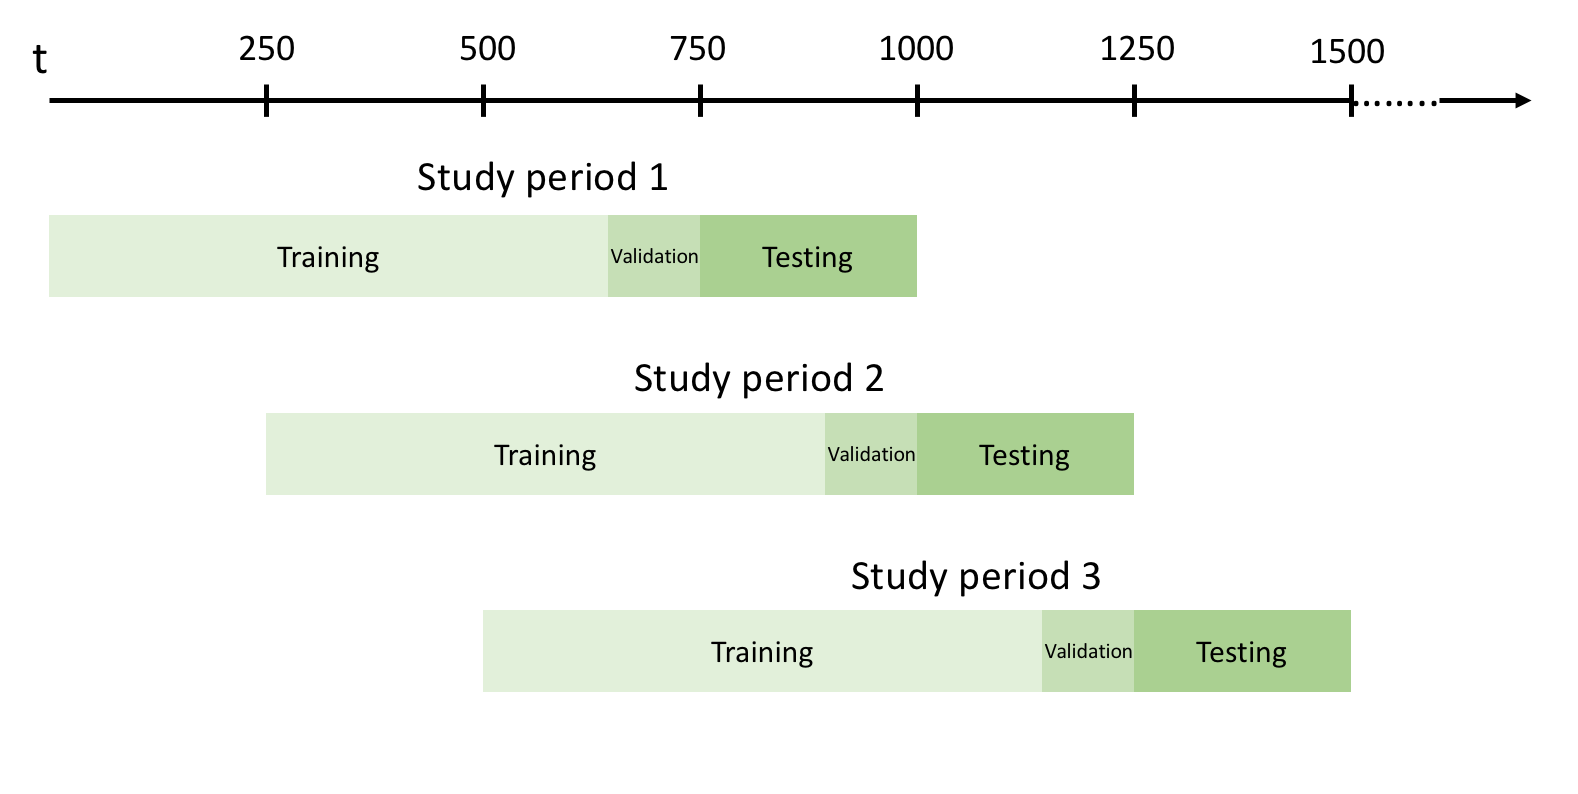
\includegraphics [scale=0.48,angle=360]{figures/study.png}
\caption{Rolling Study Periods}
\label{fig:study}
\end{figure}

\indent\newline 
Figure 4.1 illustrates the logical structure of the study periods, where the last 20\% of the training data is used for validation. Including validation sets is important in order to avoid selection bias related to the process of hyperparameters-optimization.

\indent\newline
The training and testing approach is applied to two different groups of stocks, where both groups are constituents on the Oslo Stock Exchange. The groups are constructed based on a market capitalization threshold updated at the end of each year. Small cap stocks are determined based on a market cap threshold equal to or below three billion NOK, while the threshold for large caps stocks is either equal to or above 6 billion NOK. It is difficult defining a definite threshold for what to characterize as a small cap stock and a large cap stock, but for the purpose of comparing returns between the two groups, a lower threshold is set for large cap stocks. This is a result of wanting to have a more balanced number of stocks in each group, as there are more small cap stocks listed on the Oslo Stock exchange compared to large cap stocks.  

\indent\newline
For both groups, $n_{i}$ denotes the number of stocks that are part of the groups at the last day in study period $\textit{i}$. Some of the stocks may not have a full data history for each training period, due to either being delisted or being listed at a later time. This also applies to stocks having a market cap changing above or below the thresholds during the study periods. If stocks do not exhibit share price data after a certain point in the trading period, they are included for trading up until this point. The same logic applies to stocks that are listed later than the starting point of the data, where these stocks are considered for trading after they have been listed.   

\section{Variables}
\subsection{Target Variable}
Following Krauss et al. the target variable $Y^{s}_{t + 1}$ represents a binary classification problem with two classes. The dependent variable for each stock $\textit{s}$ and date $\textit{t}$ is therefore equal to a value of either 1 or 0. This is determined on the basis of whether the one-period return $R^{1,s}_{t + 1}$ of stock $\textit{s}$ is larger or equal (class 1) to the cross-sectional median return of all stocks in period $\textit{t + 1}$, or smaller (class 0) than the cross-sectional median return. The classes are defined by ordering all one-period returns $R^{1,s}_{t + 1}$ of all stocks $\textit{s}$ in period $\textit{t + 1}$ in ascending order, and by putting them into two equally sized classes \cite{krauss}.  

\subsection{Independent Variables}
In order to improve model performance in terms of finding patterns and relationships within the data, several independent variables are used as input features for the models to train and test on. According to previous research, including a standardized one-day return with a sequence length of 240 days as a main independent variable seems to give good results with this type of neural network \cite{krauss}. To create the feature, the price process of stock $\textit{s}$ at time $\textit{t}$ is defined as $P^{s}$ = $(P^{s}_{t})_{t\in T}$ and where the simple return $R^{m,s}_{t}$ for a stock $\textit{s}$ over $\textit{m}$ periods is calculated in the following way:

\indent\newline
\begin{equation}
R^{m,s}_{t} = \frac{P^{s}_{t}}{P^{s}_{t-m}} - 1
\end{equation}

\indent\newline
The simple returns are calculated for each day and each stock $R^{1,s}_{t}$. Further, the mean and standard deviation are obtained from the training set. It is important to compute these measures only from the training set, as it ensures the network to avoid look-ahead biases. The mean $\mu^m_{train}$ is then subtracted from the simple returns and divided by the standard deviation $\sigma^{m}_{train}$ to standardize the returns:

\indent\newline
\begin{equation}
\tilde{R}^{m,s}_{t} = \frac{R^{m,s}_{t} - \mu^m_{train}}{\sigma^{m}_{train}}
\end{equation}

\indent\newline
The training process of an LSTM network requires input features to be divided into different sequences. As mentioned earlier, the standardized one-day returns $\tilde{R}^{1,s}_{t}$ have a sequence length of 240 days, which translates into approximately one year of trading. The standardized one-day returns are organized in overlapping sequences, where the feature vector is sorted by stocks $\textit{s}$ and date $\textit{t}$ in ascending order. To illustrate this, the first two sequences of the first stock $s_{1}$ have the form of $\lbrace\tilde{R}^{1,s_{1}}_{1}, \tilde{R}^{1,s_{1}}_{2}, ..., \tilde{R}^{1,s_{1}}_{240}\rbrace$ and $\lbrace\tilde{R}^{1,s_{1}}_{2}, \tilde{R}^{1,s_{1}}_{3}, ..., \tilde{R}^{1,s_{1}}_{241}\rbrace$ and so forth \cite{krauss}. 
   
\indent\newline
A large segment in the Norwegian economy is based on oil-related companies and represents a substantial part of the Oslo Stock Exchange's total market cap. Brent-crude price is therefore regarded as an important influence on the Oslo Stock Exchange and will be included as an input feature. Other independent variables that represent macroeconomic factors are the USD/NOK exchange rate and the 10-year US treasury rate, which are also included as input features. Additional input features are based on technical indicators and consist of the stock's daily volume, and moving averages with intervals of 50 and 200 days. Lastly, a measure of the broad market volatility is included as an input feature through daily data on the CBOE Volatility Index (VIX), also known as the fear index. The VIX captures market sentiment by measuring the relative strength of near-term price changes of the S\&P 500. It generates a 30-day forward projection of volatility, by being derived from prices of SPX index options with near-term expiration dates \cite{kuepper2021}.

\indent\newline
The reasoning behind including the 10-year US treasury rate and the VIX is their influence on small cap stocks. A majority of small cap stocks are not expected to generate positive cash flow before several years down the line. When investors calculate the net present value (NPV) of these companies, the rate of US treasuries affects the discount rate included in their NPV-analysis. 

\indent\newline
\begin{equation}
NPV = \sum_{t=1}^{n} \frac{R_{t}}{(1 + i)^{t}}
\end{equation}

\indent\newline
The equation above shows the formula for calculating the NPV, where $R_{t}$ is the expected net cash flow in a single time period $\textit{t}$, $\textit{i}$ is the discount rate which is based on potential returns from alternative investments, and $\textit{t}$ is the number of time periods. When investors decide on which discount rate to include in their analysis, they evaluate other returns from alternative investments. The 10-year treasury yield is a measure of a risk free rate and an alternative investment, and therefore affects the discount rate. E.g. if the risk free rate goes up, the discount rate also goes up and vice versa. A higher discount rate means that the present value of (especially) small cap stocks' future positive cash flow is negatively affected, since the positive cash flows are not expected until several years into the future. The 10-year US treasury rate should therefore, to a certain degree, explain the variability in small cap stocks' share price. Small cap stocks also tend to be more volatile than large cap stocks, which give reason to believe that the VIX could be a suitable input feature to include when predicting small cap stock returns. 

\section{Network Variations}
The following models and network-variations are included with the aim of discovering the most suitable models for predicting small cap stock returns, in order to take advantage of the excess returns that comes with this group of stocks:

\indent \newline
\begin{itemize}
\item {\textbf{LSTM all stocks:} The network trains on all stocks simultaneously with only one input feature, which consists of sequences of the last 240 stock returns. This network does not learn patterns and relationships within the data for each stock, but common relationships for all stocks.} 
\item {\textbf{LSTM stacked (2 layers):} As apposed to the previous, more basic model, this model has a network structure with two LSTM layers, which can potentially enable the network to discover deeper patterns within the data. The model trains on only the previous mentioned input feature.}
\item {\textbf{LSTM stacked (3 layers):} The network follows the same structure as the LSTM stacked, but this network has three layers to make the network even deeper. The model trains on only the main input feature.}
\item {\textbf{LSTM extra input features:} The last LSTM-variation follows the same principles as the first LSTM-network, but it trains on data with additional input features. The reasoning behind including extra input features is to help the model explain the variability in stock returns.}
\item {\textbf{GRU all stocks:} The GRU-network differs from the LSTM-network in terms of having two gates (reset and update) instead of three (input, output and forget). The model trains on all stocks simultaneously with the same main input feature as the other networks.}
\item {\textbf{GRU extra input features:} The model trains on all stocks simultaneously with additional input features, consisting of the VIX, Brent-crude oil price, 10-years US treasury yield, USD/NOK exchange rate, and 50- and 200-days moving averages.}
\end{itemize}

\section{Evaluation Metrics}
\subsection{Predictions}
Several threshold metrics for classification are used to assess and evaluate the accuracy of the networks. The section presents five performance metrics chosen on the basis of quantifying the prediction errors and accuracy of the networks, either by a fraction, ratio or rate. The first metric measures the networks' accuracy, which is the fraction of observations correctly classified:

\indent\newline
\begin{equation}
Accuracy = \frac{CP}{TP}
\end{equation}
\indent \newline 
\textit{Where,
\begin{itemize}
    \item[] $CP$ = Correct predictions
    \item[] $TP$ = Total predictions
\end{itemize}
}

\indent \newline 
The next metric is quite similar to the previous one, but instead of measuring the amount of correct predictions compared to total predictions, it compares the amount of positive/negative predictions with total positive/negative predictions:

\indent\newline
\begin{equation}
Presicion = \frac{CPP}{TPP}
\end{equation}
\indent \newline 
\textit{Where,
\begin{itemize}
    \item[] $CPP$ = Correct positive predictions
    \item[] $TPP$ = Total positive predictions
\end{itemize}
}

\indent \newline 
Another metric incorporated to evaluate network performance is recall. The measurement looks at the ratio of the networks' correct positive prediction compared to the amount of actual positive observations:

\indent\newline
\begin{equation}
Recall = \frac{CPP}{TPO}
\end{equation}
\indent \newline 
\textit{Where,
\begin{itemize}
    \item[] $CPP$ = Correct positive predictions
    \item[] $TPO$ = Total positive observations
\end{itemize}
}

\indent \newline 
The next metric is the F1-score. It uses the positive accuracy and recall to measure the networks' predictive accuracy in terms of robustness:

\indent\newline
\begin{equation}
F1-Score = \frac{P * Recall}{P + Recall}
\end{equation}
\indent \newline 
\textit{Where,
\begin{itemize}
    \item[] $P$ = Precision
\end{itemize}
}

\indent \newline 
The fifth and last evaluation metric is binary cross-entropy, which is the networks' loss function during training. In addition to measuring if predictions are correct or not, it also takes into account the difference between the predicted probabilities and actual outcomes \cite{lund}:

\indent \newline 
\begin{equation}
BCE = \frac{1}{N} \sum^{N}_{n=0} (y_{n}log[p_{n}] + (1 - y_{n})log[1 - p_{n}])
\end{equation}
\indent \newline 
\textit{Where,
\begin{itemize}
    \item[] $BCE$ = Binary cross entropy
    \item[] $N$ = Number of observations
    \item[] $y_{n}$ = Actual class of observation n
    \item[] $p_{n}$ = Predicted probability of observation n    
\end{itemize}
}

\subsection{Trading}
Multiple financial metrics are used for evaluating the trading performance of each network. These include annualized returns, standard deviation, Sharpe ratio, max drawdown, and value at risk (VaR). The chosen metrics capture both the returns from trading while also highlighting the risk associated with each model and strategy. Lastly, Jensen's Alpha (discussed in chapter two) is implemented as a measure for comparing small cap returns with large cap returns, as well as the small cap index OSESX and the Benchmark index OSEBX.  

\indent \newline 
The Sharpe ratio is a measure which highlights the level of risk compared to returns. It is a ratio of average return earned in excess of the risk-free rate per unit of total risk or volatility \cite{fernando}. When analyzing the returns from trading in small caps and large caps, It is important to balance the results by not only comparing returns between the groups, but also the level of portfolio risk. Sharpe ratio is calculated in the following way:

\indent \newline
\begin{equation}
SR = \frac{R_{p} - R_{f}}{\sigma_{p}}
\end{equation}
\indent \newline 
\textit{Where,}
\indent \newline 
$SR$ = Sharpe ratio
\indent \newline 
$R_{p}$ = Return of portfolio
\indent \newline 
$R_{f}$ = Risk-free rate
\indent \newline 
$\sigma_{p}$ = Standard deviation of the portfolio's excess returns

\indent \newline 
Maximum drawdown is included to assess the portfolios' maximum observed loss from a peak to a trough, before attaining a new peak \cite{hayes}. In other words, it measures the greatest movement from a high point to a low point, which can interpreted as a representation of volatility and especially downside risk:

\indent \newline
\begin{equation}
MDD = \frac{TV - PV}{PV}
\end{equation}
\indent \newline 
\textit{Where,}
\indent \newline 
$MDD$ = Maximum drawdown
\indent \newline 
$TV$ = Trough value
\indent \newline 
$PV$ = Peak value

\indent \newline
Lastly, the value at risk (VaR) measures potential losses in a portfolio and their occurrence ratio. Volatility by itself is not a sufficient measure, as it does not differentiate between stocks with small fluctuations downwards in share price, but large fluctuations up in share price and vice versa. VaR addresses this issue by quantifying the risk of potential downside in a given stock. It is specifically directed towards the chance of experiencing big losses.  

\section{Benchmarks}
To be able to adequately assess and evaluate the application of the proposed models to small cap trading, it requires having suitable points of references. The models' training, testing and predictions on large cap stock returns serves as benchmarks for the models and strategies applied to predicting small cap stock returns. Hence, each model and trading strategy is tested on both groups of stocks for comparison reasons. Most investors compare their portfolio returns with other diversified "portfolios" such as indices, in order to evaluate portfolio performance. Following this approach for evaluating portfolio performance, the returns of the small cap index OSESX and the benchmark index OSEBX in the corresponding periods are also incorporated as benchmark measures. The performance of all stocks in the small cap data set and large cap data set is also incorporated as benchmarks. 

\section{Strategies}
The models predict the probability $\widehat{\mathcal{P}}^{s}_{t+1|t}$ of a stock outperforming or underperforming the cross-sectional median return, where the models only use information up until time $\textit{t}$. For each period $\textit{t+1}$, the stocks are ranked in descending order based on their respective probability. The top of the ranking corresponds to the stocks the models evaluate as undervalued with expectations to outperform the cross-sectional median return, and is the basis for which stocks to buy. The bottom of the ranking corresponds to the stocks the models evaluate as overvalued with expectations of underperforming the cross-sectional median return, and dictates which stocks to short. This approach makes for several different portfolio strategies, where the models are instructed to buy (short) $\textit{K}$ stocks. The following portfolio strategies are selected:

\indent \newline
\begin{itemize}
\item {\textbf{Long-only portfolio:} The strategy involves being only long in $\textit{K}$ stocks. This means that shorting is not allowed. Two long-only portfolios are selected, where one is instructed to hold five stocks at any given time (K=5), and the other is instructed to hold two stocks (K=2).} 
\item {\textbf{Long-short portfolio:} This strategy replicates a common portfolio for professional investors. The strategy allows for going both long and short. The models are instructed to create a portfolio consisting of being long five stocks and being short five stocks (2K, K=5) at any given point.}
\item {\textbf{Short-only portfolio:} The last strategy involves an unconventional trading approach, by only allowing for short-selling. The models create a portfolio of the most overvalued stocks (based on the probability of underperforming the cross-sectional median return) and are instructed to hold five short positions at any given time (K=5).}
\end{itemize}  

\indent \newline
The main portfolio strategy applied to every model is the long-only portfolio with K=5. The other strategies are only applied to the LSTM network that is trained on all stocks, with a single independent input feature of the previous 240 stock returns. All models and portfolio strategies are first assessed and evaluated without taking into account transaction costs, before including explicit transaction costs in the form of broker commissions. Transaction costs related to securities lending for short-selling and the implicit costs of the bid-ask spread (arrival costs) are not included in the backtesting. However, these costs are discussed on the basis of previous research, in order to give an overall assessment of how the different models and strategies perform when applied to real-life trading. An assumption for each model and portfolio strategy is that 100\% of the capital is invested at all times during the trading period. Bet sizing is simplified by using equal-weighted portfolios, which means that the amount of capital invested in each stock is equal for all stocks the models suggest to invest in. 